
\section{Deliverable 4: Differences in cost function (Circle dataset)}


\begin{solve}    

\begin{figure}[H]
    \centering
    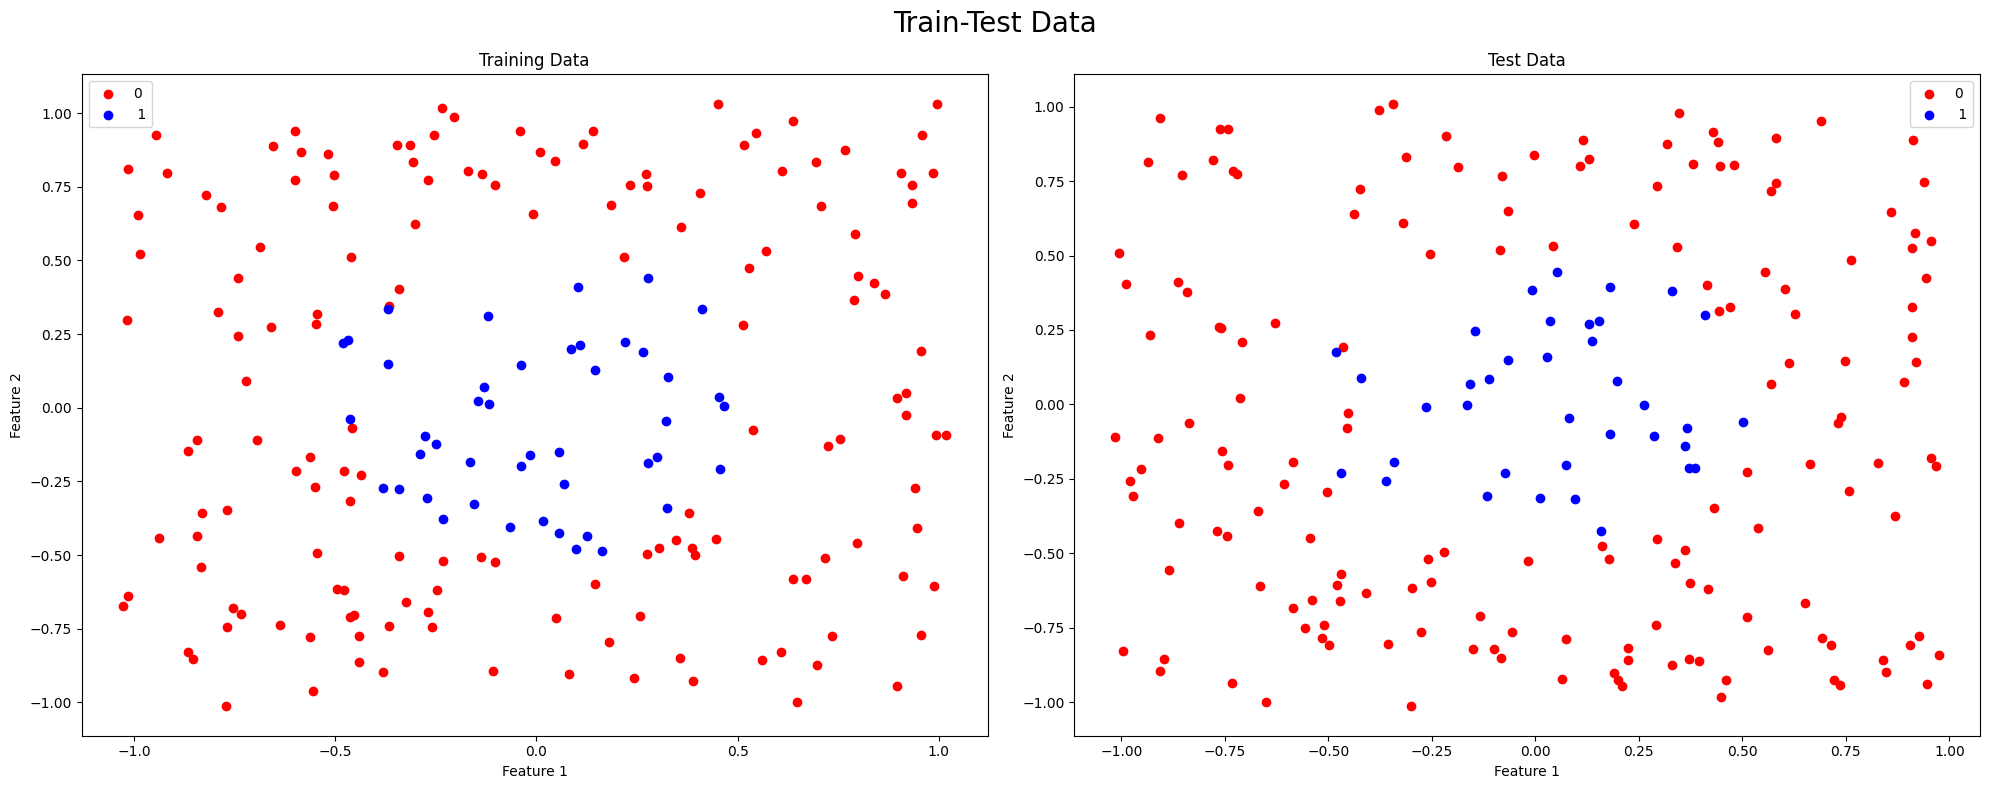
\includegraphics[width=0.7\textwidth]{plots/4_circle_dataset.png}
    \caption{Circle dataset (train, test set with 200 points each)}
\end{figure}

\subsection*{Key Differences Noted}
\begin{itemize}
    \item The decision boundary for the L2Loss is less smooth compared to the CrossEntropyLoss. This is because the L2Loss is a regression loss and the CrossEntropyLoss is a classification loss.
    \item Related to the above point, the L2Loss decision boundary seems more oval than the one from CrossEntropyLoss, which is more circular (hence closer to the actual decision boundary).
    \item Final Accuracy and loss are the same, however, we see the L2Loss has a more jittery loss graph compared to the CrossEntropyLoss, evident in the spikes in the loss graph.
\end{itemize}


\subsection{L2Loss}

\begin{lstlisting}[language=python]
# one hot encoding the output to get the final output (dim 1 for prediction)
dim_in, dim_out = x_train.shape[1], 2
hidden_neuron_list = [4,16]
# ReLU was giving similar accuracy but more boxy decision boundary
activation_list = ['Tanh', 'Tanh','Sigmoid']
opt_init = 'xavier'
opt_loss = L2Loss()
mlp = MLP(dim_in, dim_out, hidden_neuron_list, activation_list, opt_init)
opt_optim = Adam(mlp)
print(mlp.summary())
-----------------------------------------------------------------
Model Summary
-------------
Layer 1: Linear - A Dim: 2, Output Dim: 4, Parameters: 12
Layer 2: Tanh
Layer 3: Linear - A Dim: 4, Output Dim: 16, Parameters: 80
Layer 4: Tanh
Layer 5: Linear - A Dim: 16, Output Dim: 2, Parameters: 34
Layer 6: Sigmoid
Total Parameters: 126
\end{lstlisting}

\begin{figure}[H]
    \centering
    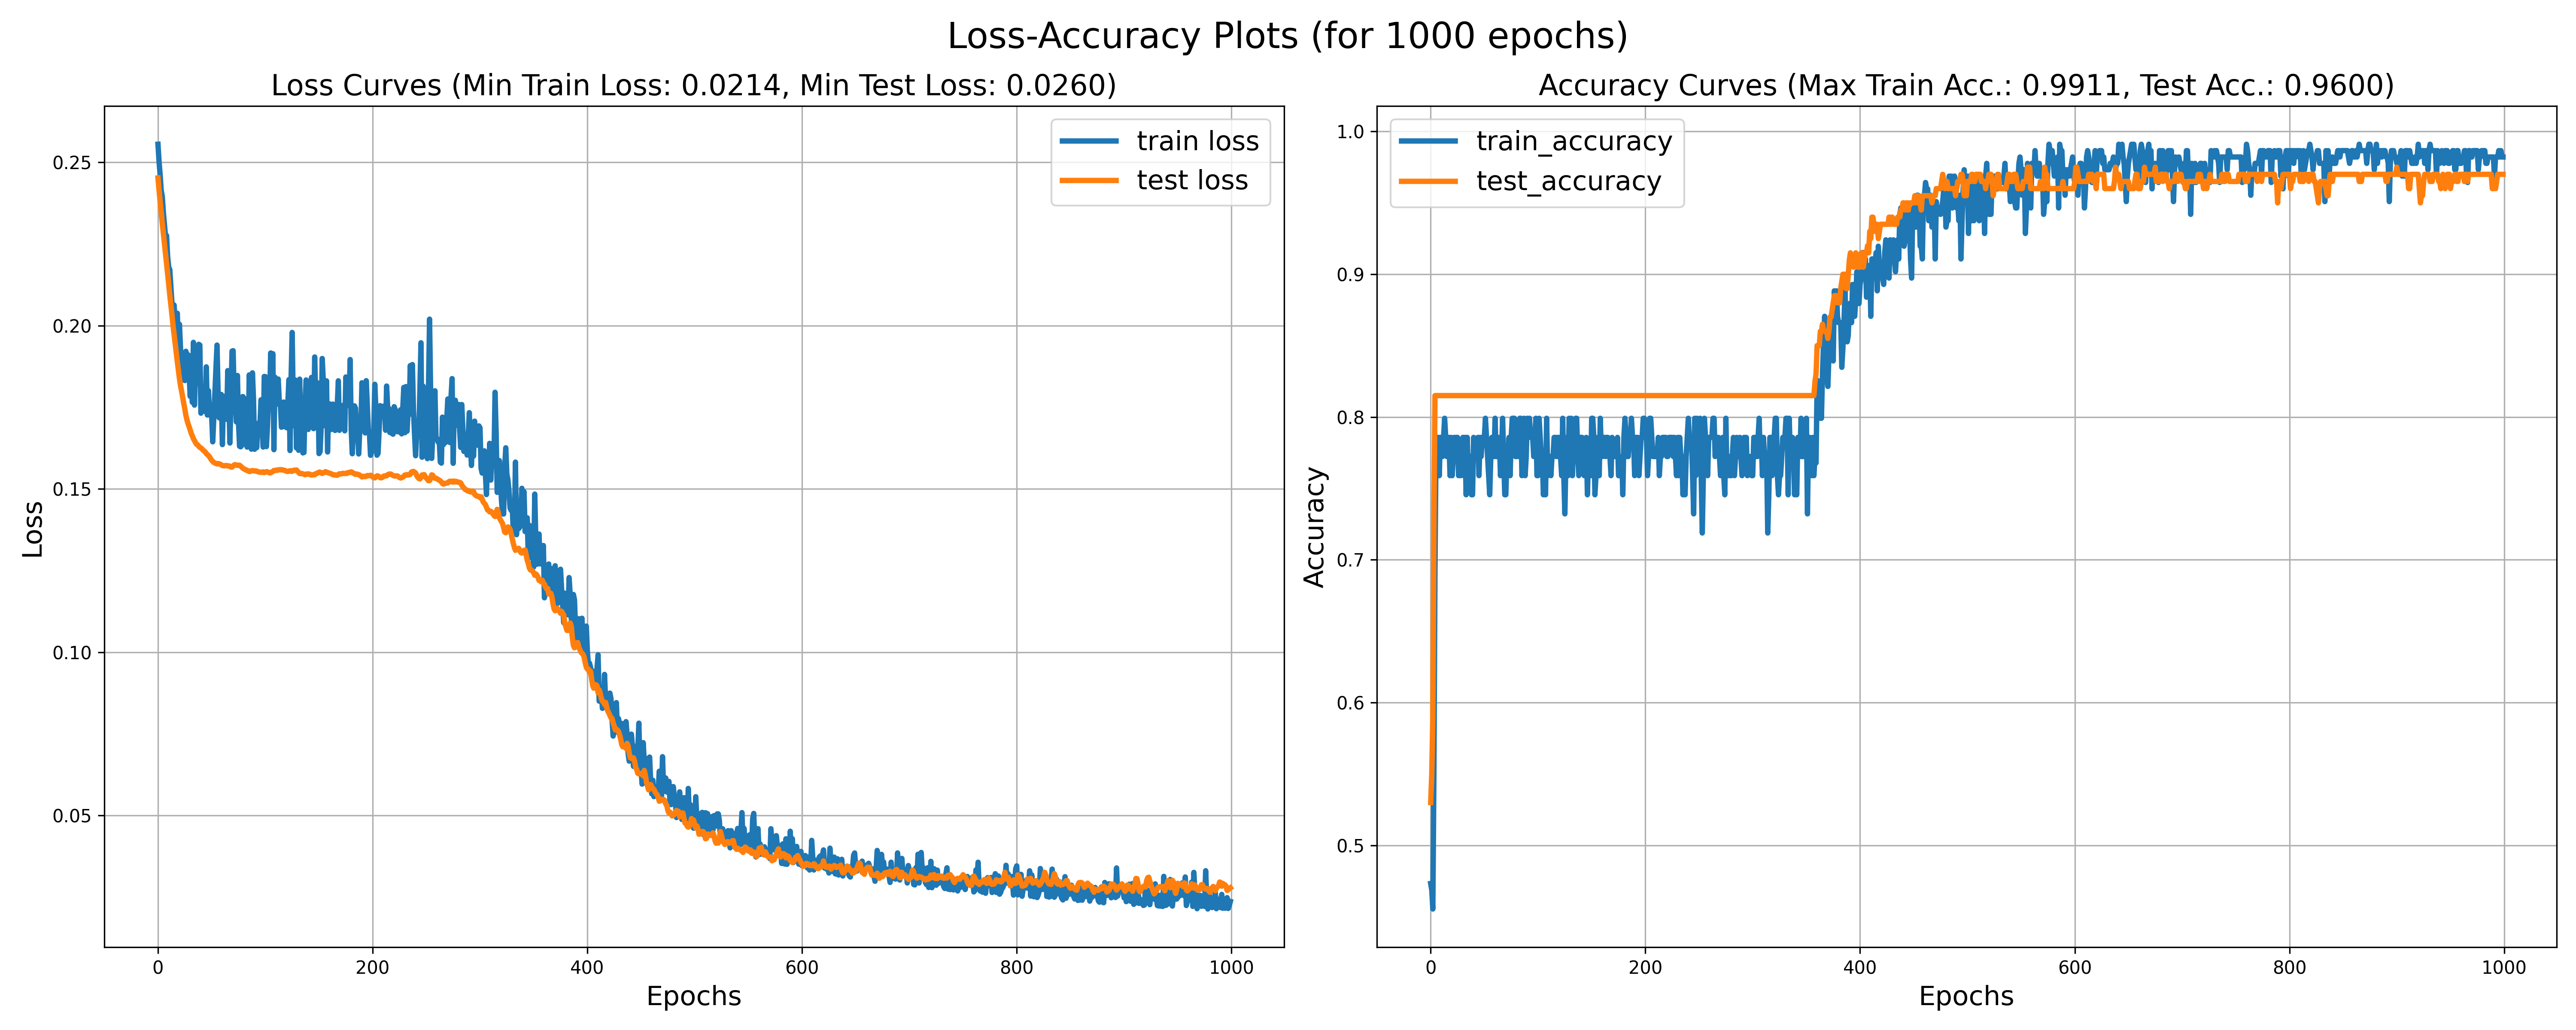
\includegraphics[width=0.9\textwidth]{plots/4_circle_adam_regressionloss_acc.png}
    \caption{Loss and accuracy for Circle dataset (train, test set with 200 points each), Adam optimizer, 500 epochs, Cost function: L2Loss, Xaiver initialization}
\end{figure}

\begin{figure}[H]
    \centering
    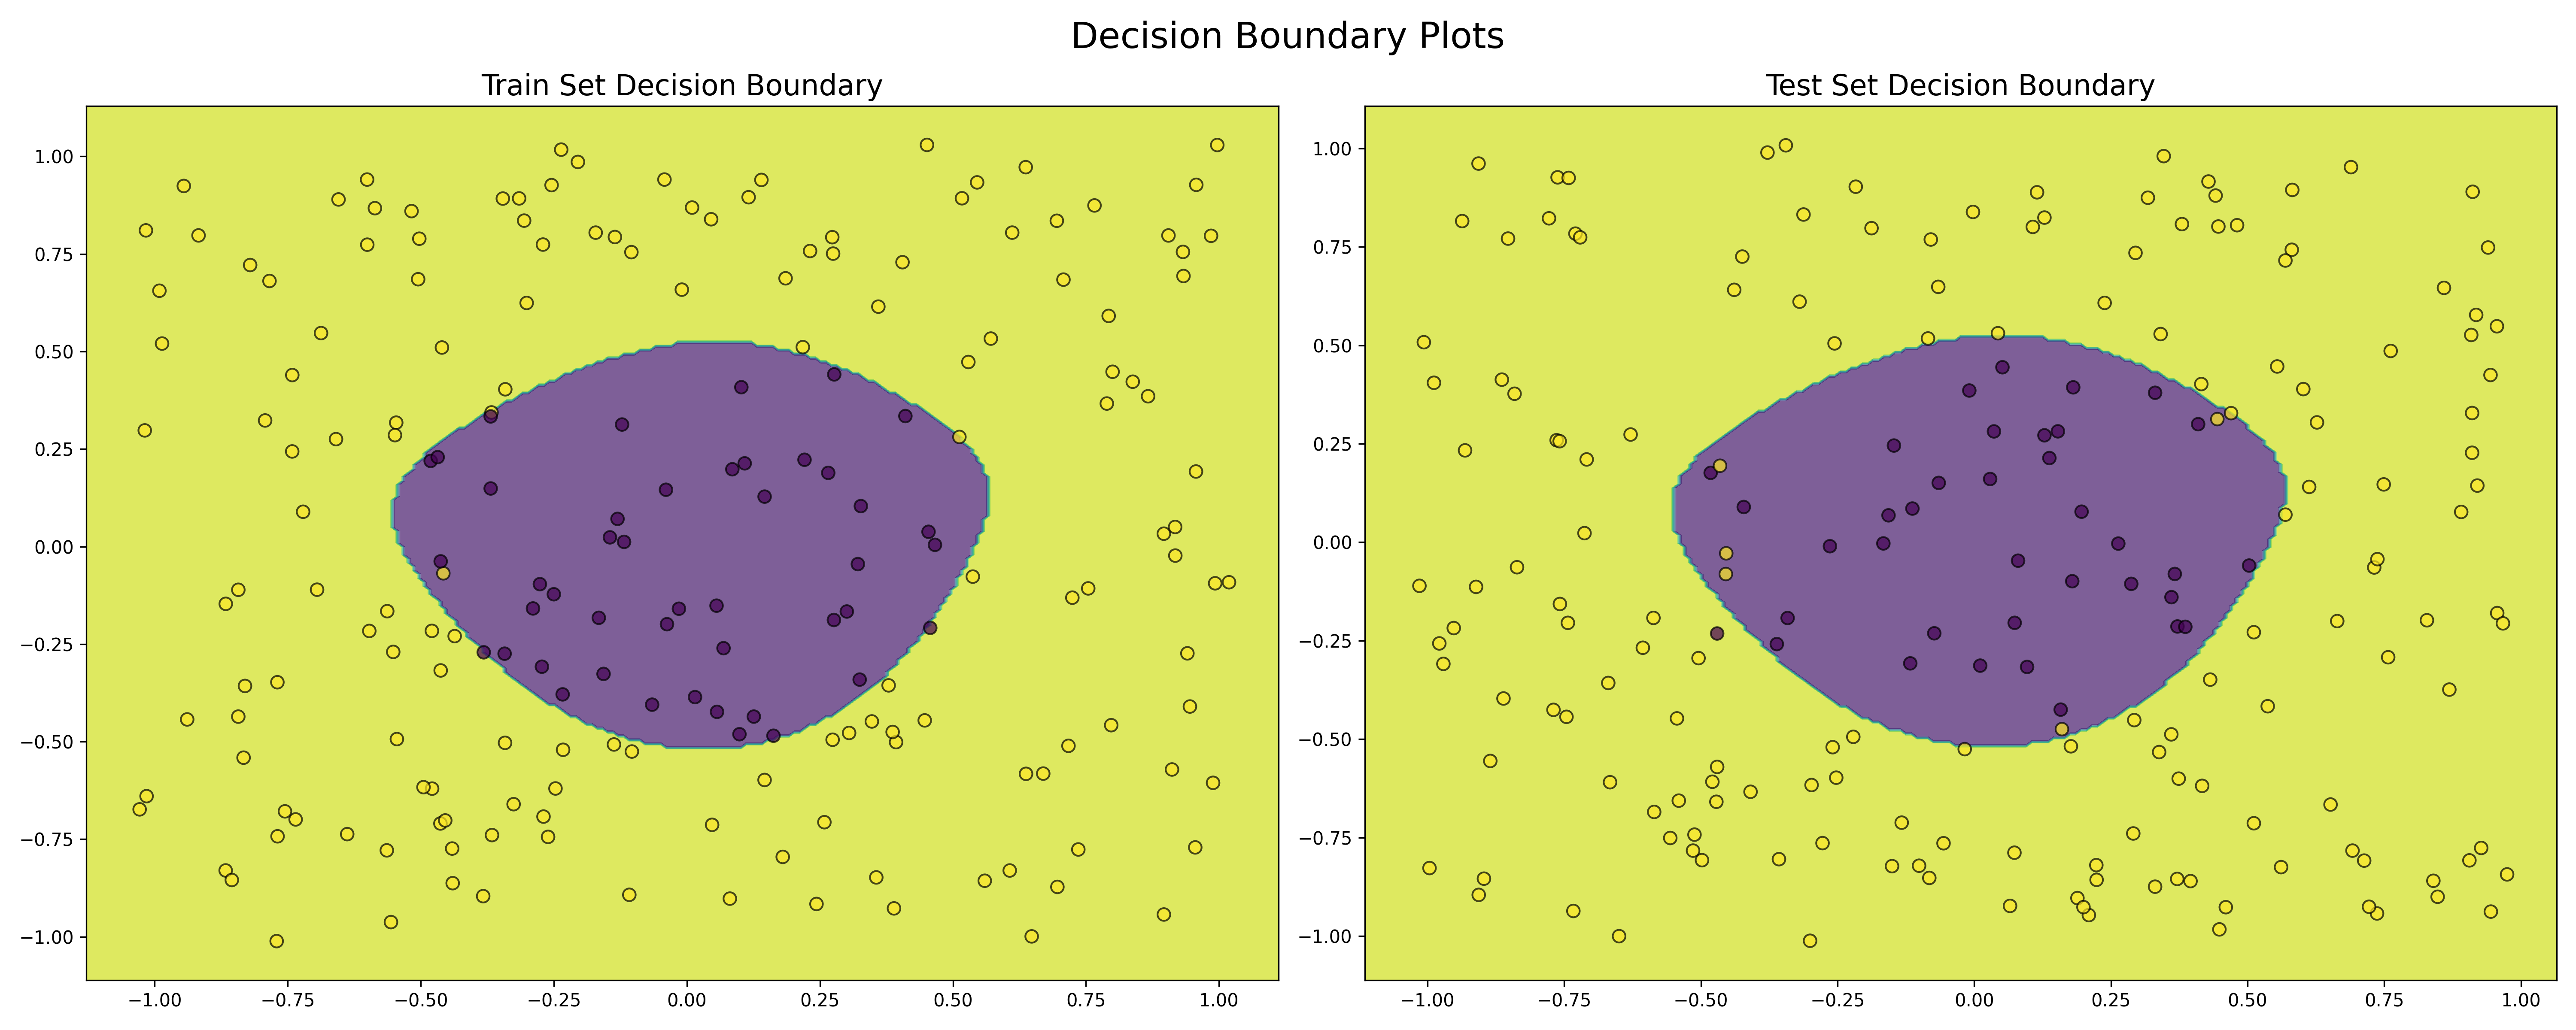
\includegraphics[width=0.8\textwidth]{plots/4_circle_adam_regressionboundary.png}
    \caption{(L2Loss) Decision boundary for Circle separable dataset (train, test set with 200 points each)}
\end{figure}

% ############################################

\subsection{CrossEntropyLoss}

\begin{lstlisting}[language=python]
    dim_in, dim_out = x_train.shape[1], 2
hidden_neuron_list = [4,16]
# LinearActivation used in the last layer because sigmoiding in the loss function forward pass

activation_list = ['Tanh', 'Tanh','LinearActivation']
opt_init = 'xavier'
opt_loss = CrossEntropyLoss()
mlp = MLP(dim_in, dim_out, hidden_neuron_list, activation_list, opt_init)
opt_optim = Adam(mlp)
print(mlp.summary())
-----------------------------------------------------------------
Model Summary
-------------
Layer 1: Linear - A Dim: 2, Output Dim: 4, Parameters: 12
Layer 2: Tanh
Layer 3: Linear - A Dim: 4, Output Dim: 16, Parameters: 80
Layer 4: Tanh
Layer 5: Linear - A Dim: 16, Output Dim: 2, Parameters: 34
Layer 6: LinearActivation
Total Parameters: 126
\end{lstlisting}

\begin{figure}[H]
    \centering
    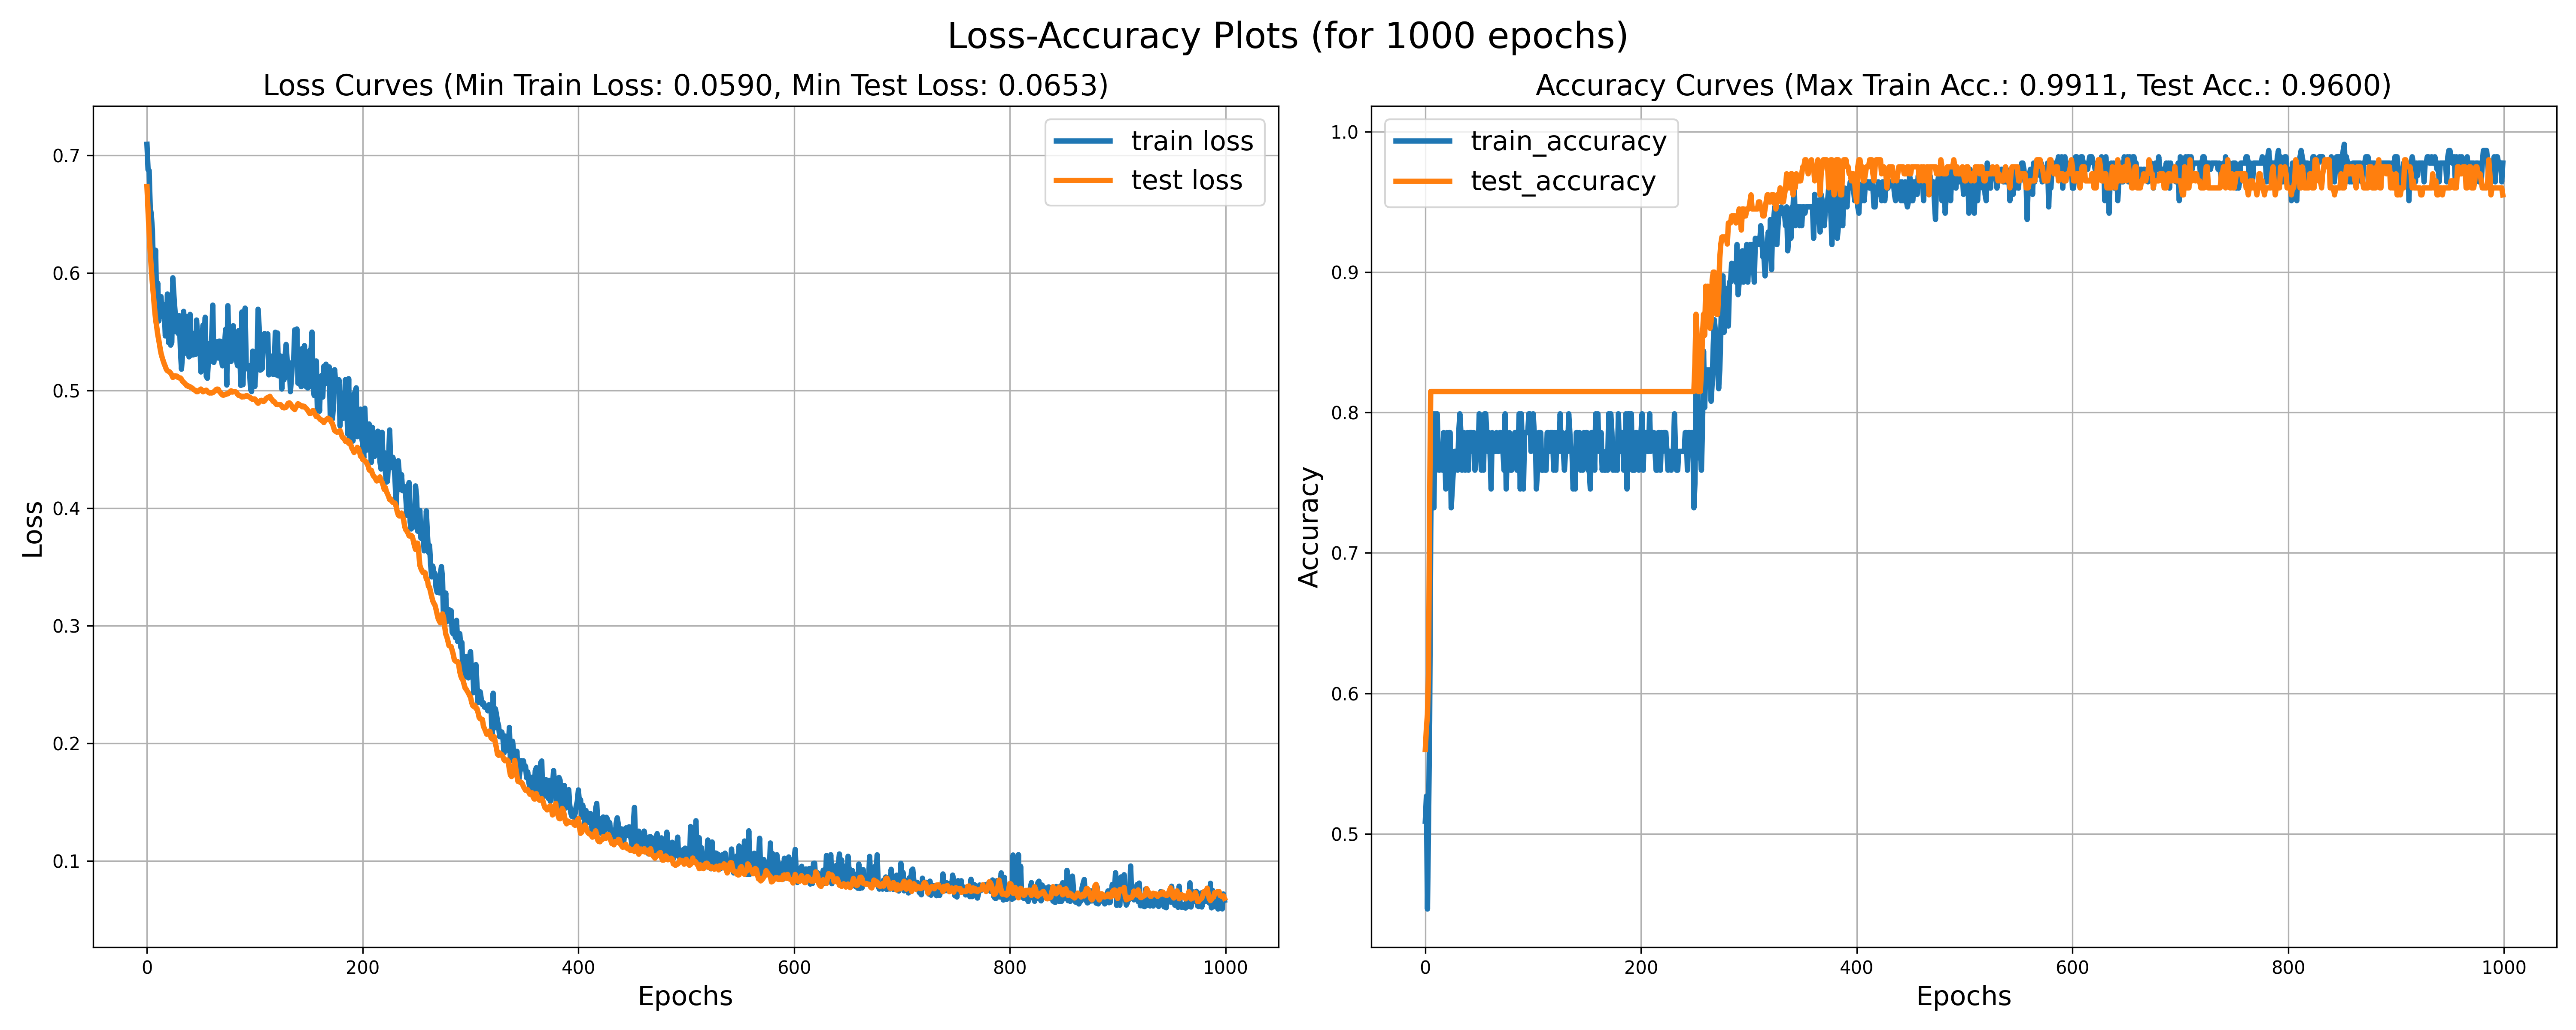
\includegraphics[width=0.9\textwidth]{plots/4_circle_adam_classificationloss_acc.png}
    \caption{Loss and accuracy for Circle dataset (train, test set with 200 points each), Adam optimizer, 500 epochs, Cost function: CrossEntropyLoss, Xaiver initialization}
\end{figure}

\begin{figure}[H]
    \centering
    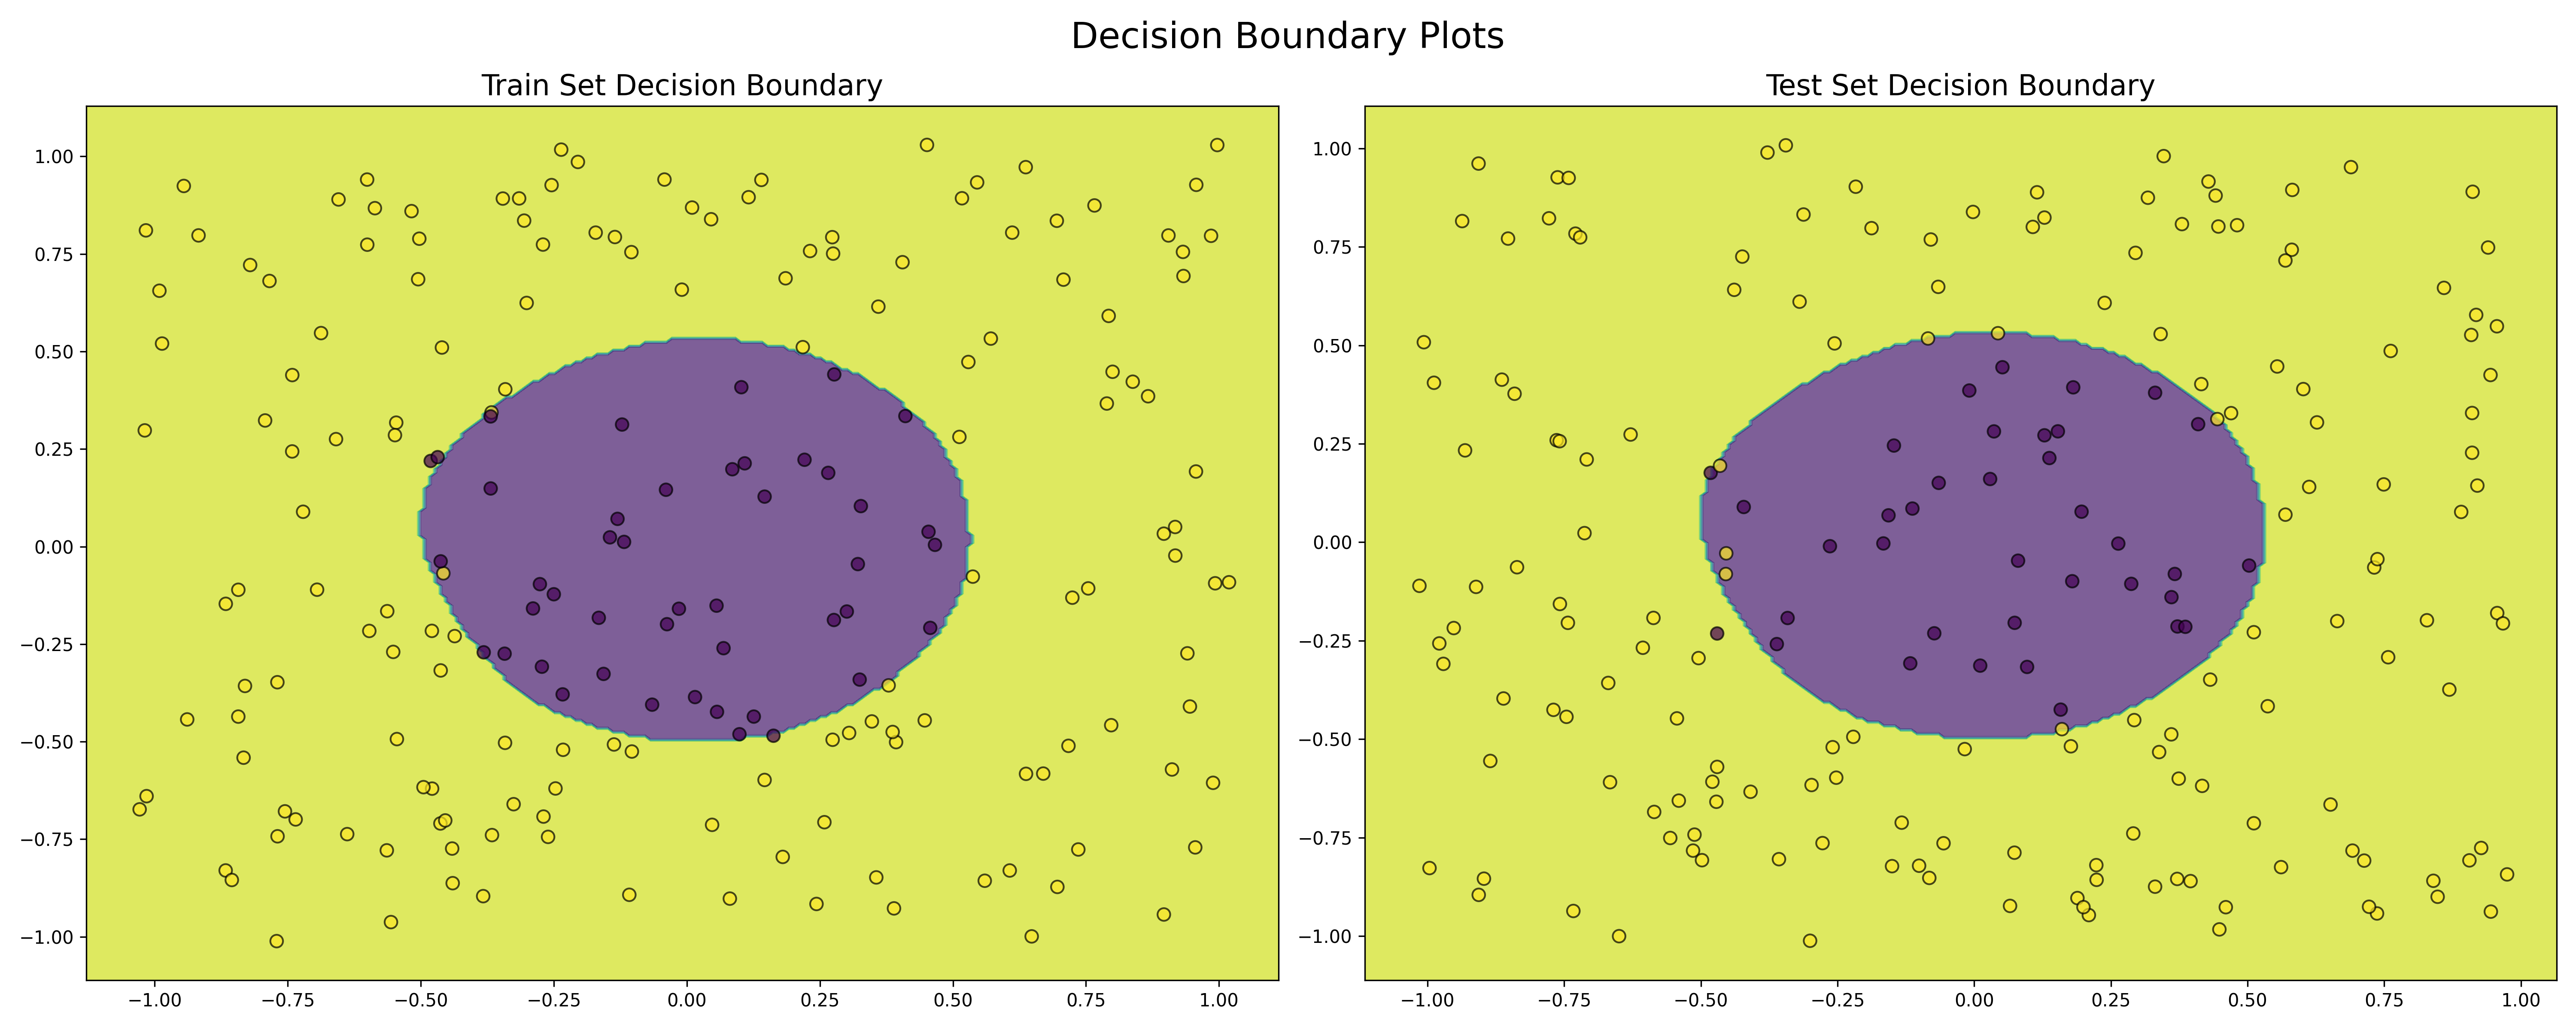
\includegraphics[width=0.8\textwidth]{plots/4_circle_adam_classificationboundary.png}
    \caption{(CrossEntropyLoss) Decision boundary for Circle separable dataset (train, test set with 200 points each)}
\end{figure}

\end{solve}
